% Options for packages loaded elsewhere
\PassOptionsToPackage{unicode}{hyperref}
\PassOptionsToPackage{hyphens}{url}
%
\documentclass[
  man]{apa6}
\usepackage{amsmath,amssymb}
\usepackage{iftex}
\ifPDFTeX
  \usepackage[T1]{fontenc}
  \usepackage[utf8]{inputenc}
  \usepackage{textcomp} % provide euro and other symbols
\else % if luatex or xetex
  \usepackage{unicode-math} % this also loads fontspec
  \defaultfontfeatures{Scale=MatchLowercase}
  \defaultfontfeatures[\rmfamily]{Ligatures=TeX,Scale=1}
\fi
\usepackage{lmodern}
\ifPDFTeX\else
  % xetex/luatex font selection
\fi
% Use upquote if available, for straight quotes in verbatim environments
\IfFileExists{upquote.sty}{\usepackage{upquote}}{}
\IfFileExists{microtype.sty}{% use microtype if available
  \usepackage[]{microtype}
  \UseMicrotypeSet[protrusion]{basicmath} % disable protrusion for tt fonts
}{}
\makeatletter
\@ifundefined{KOMAClassName}{% if non-KOMA class
  \IfFileExists{parskip.sty}{%
    \usepackage{parskip}
  }{% else
    \setlength{\parindent}{0pt}
    \setlength{\parskip}{6pt plus 2pt minus 1pt}}
}{% if KOMA class
  \KOMAoptions{parskip=half}}
\makeatother
\usepackage{xcolor}
\usepackage{graphicx}
\makeatletter
\def\maxwidth{\ifdim\Gin@nat@width>\linewidth\linewidth\else\Gin@nat@width\fi}
\def\maxheight{\ifdim\Gin@nat@height>\textheight\textheight\else\Gin@nat@height\fi}
\makeatother
% Scale images if necessary, so that they will not overflow the page
% margins by default, and it is still possible to overwrite the defaults
% using explicit options in \includegraphics[width, height, ...]{}
\setkeys{Gin}{width=\maxwidth,height=\maxheight,keepaspectratio}
% Set default figure placement to htbp
\makeatletter
\def\fps@figure{htbp}
\makeatother
\setlength{\emergencystretch}{3em} % prevent overfull lines
\providecommand{\tightlist}{%
  \setlength{\itemsep}{0pt}\setlength{\parskip}{0pt}}
\setcounter{secnumdepth}{-\maxdimen} % remove section numbering
% Make \paragraph and \subparagraph free-standing
\makeatletter
\ifx\paragraph\undefined\else
  \let\oldparagraph\paragraph
  \renewcommand{\paragraph}{
    \@ifstar
      \xxxParagraphStar
      \xxxParagraphNoStar
  }
  \newcommand{\xxxParagraphStar}[1]{\oldparagraph*{#1}\mbox{}}
  \newcommand{\xxxParagraphNoStar}[1]{\oldparagraph{#1}\mbox{}}
\fi
\ifx\subparagraph\undefined\else
  \let\oldsubparagraph\subparagraph
  \renewcommand{\subparagraph}{
    \@ifstar
      \xxxSubParagraphStar
      \xxxSubParagraphNoStar
  }
  \newcommand{\xxxSubParagraphStar}[1]{\oldsubparagraph*{#1}\mbox{}}
  \newcommand{\xxxSubParagraphNoStar}[1]{\oldsubparagraph{#1}\mbox{}}
\fi
\makeatother
\ifLuaTeX
\usepackage[bidi=basic]{babel}
\else
\usepackage[bidi=default]{babel}
\fi
\babelprovide[main,import]{english}
% get rid of language-specific shorthands (see #6817):
\let\LanguageShortHands\languageshorthands
\def\languageshorthands#1{}
% Manuscript styling
\usepackage{upgreek}
\captionsetup{font=singlespacing,justification=justified}

% Table formatting
\usepackage{longtable}
\usepackage{lscape}
% \usepackage[counterclockwise]{rotating}   % Landscape page setup for large tables
\usepackage{multirow}		% Table styling
\usepackage{tabularx}		% Control Column width
\usepackage[flushleft]{threeparttable}	% Allows for three part tables with a specified notes section
\usepackage{threeparttablex}            % Lets threeparttable work with longtable

% Create new environments so endfloat can handle them
% \newenvironment{ltable}
%   {\begin{landscape}\centering\begin{threeparttable}}
%   {\end{threeparttable}\end{landscape}}
\newenvironment{lltable}{\begin{landscape}\centering\begin{ThreePartTable}}{\end{ThreePartTable}\end{landscape}}

% Enables adjusting longtable caption width to table width
% Solution found at http://golatex.de/longtable-mit-caption-so-breit-wie-die-tabelle-t15767.html
\makeatletter
\newcommand\LastLTentrywidth{1em}
\newlength\longtablewidth
\setlength{\longtablewidth}{1in}
\newcommand{\getlongtablewidth}{\begingroup \ifcsname LT@\roman{LT@tables}\endcsname \global\longtablewidth=0pt \renewcommand{\LT@entry}[2]{\global\advance\longtablewidth by ##2\relax\gdef\LastLTentrywidth{##2}}\@nameuse{LT@\roman{LT@tables}} \fi \endgroup}

% \setlength{\parindent}{0.5in}
% \setlength{\parskip}{0pt plus 0pt minus 0pt}

% Overwrite redefinition of paragraph and subparagraph by the default LaTeX template
% See https://github.com/crsh/papaja/issues/292
\makeatletter
\renewcommand{\paragraph}{\@startsection{paragraph}{4}{\parindent}%
  {0\baselineskip \@plus 0.2ex \@minus 0.2ex}%
  {-1em}%
  {\normalfont\normalsize\bfseries\itshape\typesectitle}}

\renewcommand{\subparagraph}[1]{\@startsection{subparagraph}{5}{1em}%
  {0\baselineskip \@plus 0.2ex \@minus 0.2ex}%
  {-\z@\relax}%
  {\normalfont\normalsize\itshape\hspace{\parindent}{#1}\textit{\addperi}}{\relax}}
\makeatother

\makeatletter
\usepackage{etoolbox}
\patchcmd{\maketitle}
  {\section{\normalfont\normalsize\abstractname}}
  {\section*{\normalfont\normalsize\abstractname}}
  {}{\typeout{Failed to patch abstract.}}
\patchcmd{\maketitle}
  {\section{\protect\normalfont{\@title}}}
  {\section*{\protect\normalfont{\@title}}}
  {}{\typeout{Failed to patch title.}}
\makeatother

\usepackage{xpatch}
\makeatletter
\xapptocmd\appendix
  {\xapptocmd\section
    {\addcontentsline{toc}{section}{\appendixname\ifoneappendix\else~\theappendix\fi: #1}}
    {}{\InnerPatchFailed}%
  }
{}{\PatchFailed}
\makeatother
\keywords{lateralization, formants, variation, linguistic constraints}
\DeclareDelayedFloatFlavor{ThreePartTable}{table}
\DeclareDelayedFloatFlavor{lltable}{table}
\DeclareDelayedFloatFlavor*{longtable}{table}
\makeatletter
\renewcommand{\efloat@iwrite}[1]{\immediate\expandafter\protected@write\csname efloat@post#1\endcsname{}}
\makeatother
\usepackage{csquotes}
\ifLuaTeX
  \usepackage{selnolig}  % disable illegal ligatures
\fi
\usepackage{bookmark}
\IfFileExists{xurl.sty}{\usepackage{xurl}}{} % add URL line breaks if available
\urlstyle{same}
\hypersetup{
  pdftitle={Lateralization of the syllable-final /r/ to /l/ in the Puerto Rican diaspora},
  pdfauthor={Yhosep Barba1},
  pdflang={en-EN},
  pdfkeywords={lateralization, formants, variation, linguistic constraints},
  hidelinks,
  pdfcreator={LaTeX via pandoc}}

\title{Lateralization of the syllable-final /r/ to /l/ in the Puerto Rican diaspora}
\author{Yhosep Barba\textsuperscript{1}}
\date{}


\shorttitle{Lateralization of the /r/ in the Puerto Rican Diaspora}

\authornote{

Yhosep Barba is a PhD student in the Department of Spanish and Portuguese at Rutgers University.

The authors made the following contributions. Yhosep Barba: Conceptualization, Writing - Original Draft Preparation, Writing - Review \& Editing.

Correspondence concerning this article should be addressed to Yhosep Barba. E-mail: \href{mailto:y.barba@rutgers.edu}{\nolinkurl{y.barba@rutgers.edu}}

}

\affiliation{\vspace{0.5cm}\textsuperscript{1} Rutgers University}

\abstract{%
Early studies on the lateralization of the Puerto Rican /r/ to {[}l{]} (e.g., López Mórales, 1992) described the phenomenon categorically, with words like puerto {[}pwél.to{]} (`port') and verde {[}'bel.de{]} (`green') showing clear neutralization. Nonetheless, recent research supports a gradient approach to lateralization (Luna, 2010), indicating that lateralized /ɾ/ typically has F3 values 500--1000 Hz lower and F4 values about 120 Hz lower than canonical {[}l{]}. In this study, I examine the lateralization of the syllable-final /ɾ/ in Puerto Ricans living in New Jersey, with a focus on how linguistic and social constraints influence its production. Using the Montreal Forced-Aligner (McAuliffe et al., 2017), I analyze 420 tokens of syllable-final /ɾ/ from 14 participants, measuring F3 and F4 frequencies. The results reveal that both internal linguistic factors (such as word position and preceding vowel) and external social factors (notably gender) significantly affect lateralization. Specifically, word-final position consistently led to lower F3 and F4 values, while the preceding vowel influenced both formants: vowel /o/ lowered F3 but had no significant effect on F4, while vowel /e/ raised both formants, particularly in interaction with gender. Gender emerged as a strong predictor, with women producing higher F3 and F4 values compared to men, and this effect was further modulated by vowel quality, particularly /e/ and /o/. Educational background showed a descriptive link to lower F3 and F4 values among more educated participants, though group imbalances limited formal statistical testing.
}



\begin{document}
\maketitle

\begin{center}\rule{0.5\linewidth}{0.5pt}\end{center}

\section{Methods}\label{methods}

\subsection{Participants}\label{participants}

The data for this study was collected through a series of individual online interviews conducted between January and April 2025 in New Jersey. These interviews, each lasting about an hour, were done in Spanish with 14 Puerto Rican participants living across the state. This study included 7 self-identified women and 7 self-identified men, their ages ranged from 26 to 70 years old (the average age was 44.21 years with a standard deviation of 17.34), which indicates a wide range of generational experiences. Participants had varying levels of education background: most held college or graduate degrees, with 5 having completed doctoral programs, two with a master's degree, 6 with a bachelor's degrees, and 1 with a high school diploma. The amount of time participants had lived in New Jersey ranged from 3 to 66 years, reflecting both recent arrivals and long-term residents in the state.

\subsection{Material}\label{material}

Throughout the interviews, four materials were used: (1)a linguistic and background questionnaire, (2) open-ended questions on topics such as holidays, description of Spanish-speaking communities in their neighborhoods, and migration experiences, (3)a reading task and (4) a series of metalinguistic, open-ended questions aimed at exploring daily interactions with linguistic ideologies, metapragmatic awareness of (non)accommodation, and pride in their Puerto Rican linguistic repertoire. For this exercise, I will describe only the reading task section (tool that it was used to get participant's F3 and F4 measurements).

\subsection{La Historia de Juan (`The Story of Juan')}\label{la-historia-de-juan-the-story-of-juan}

The fictional narrative La historia de Juan is a 301-word story created with the assistance of ChatGPT (OpenAI). This narrative was specifically designed to include a range of phonological and morphological contexts relevant to the lateralization of syllable-final /ɾ/ to {[}l{]}, a key focus of this study.
A total of 30 tokens in the story featured syllable-final /ɾ/ in positions where lateralization could potentially occur. Of these, 17 tokens (56.7\%) occurred in word-final position, while 13 tokens (43.3\%) were in word-internal position. The phonological environment was carefully balanced, with 12 tokens (40\%) preceding the vowel /a/, 11 tokens (36.7\%) preceding /e/, and 7 tokens (23.3\%) preceding /o/.
Morphological category was also considered during the design of the narrative. Among the 30 relevant tokens, 12 (40\%) were nouns, 11 (36.7\%) were verbs, 6 (20\%) were adjectives, and 1 (3.3\%) was a preposition. These distributions allowed for analysis of how both linguistic and morphosyntactic contexts may influence the realization of lateralized /ɾ/.

\subsection{Procedure}\label{procedure}

Each interview was divided into five parts. First, participants were reminded of their rights and privacy protections. They then completed the Linguistic History Questionnaire (25 minutes), which was not recorded. For four participants who had difficulty, I assisted by reading the questions aloud and recording their responses.
Next, the recorded part of the interview included three tasks: a set of open-ended questions, a reading task, and a second set of open-ended questions. The first set focused on personal topics to build rapport and reduce tension. The reading task, La historia de Juan, was placed after the initial questions to mitigate style-shifting effects and allow participants to feel more at ease. Finally, participants answered questions about their linguistic experiences and perceptions.

\subsection{Data analysis}\label{data-analysis}

30 words from the fictional narrative that could have led to the lateralization of the /r/ into {[}l{]} in coda position were forced aligned using the Montreal Forced-Aligner (McAuliffe et al., 2017). For example, if a word like puerta {[}pwél.ta{]} (`door') was found in the data, it was segmented into its corresponding sounds, {[}p{]} {[}w{]} {[}é{]} {[}l{]} {[}t{]} {[}a{]}. This yielded a total of 420 tokens across the 14 participants: 182 in word internal position, and 238 in word final position. After examining the forced aligned segmentation manually to ensure accuracy, I used a Praat script (Bland, 2025) to calculate and extract the average third and fourth formant frequencies (henceforth F3 and F4) for the lateralized /r/ tokens across the duration of the segment, as well as at the mid-point. This yielded a total of 1680 segmental measurements for coda /r/, including 840 F3 measurements (420 average measurements and 420 midpoint measurements) and 840 F4 measurements (420 average measurements and 420 midpoint measurements).

\section{Results}\label{results}

The results are presented in two sections. The first addresses the initial research question, which aims to provide a general overview on the results of F3 and F4 measurements across participants. The second section examines the influence of linguistic factors (word position, preceding vowel, and word category) and social variables (gender and educational background) on F3 and F4 values.
With the exception of the first section, the analysis includes results from a mixed-effects model conducted in R (R Core Team, 2025), which evaluates the impact of the relevant linguistic and extralinguistic variables. Descriptive statistics and visualizations generated with the ggplot2 package (Wickham et al., 2025) are also provided to illustrate the direction of significant effects.

\subsection{General Statistical Analysis}\label{general-statistical-analysis}

To start with, it is important to note that averages and standard deviation results, in this section, were calculated using the mean() and sd() functions in R, which summarized the F3 and F4 values at the midpoint and across the entire segment. When looking at all participants together, the mean F3 value at the midpoint of the segment was 2417.93 Hz (SD = 425.41 Hz), while the mean for the entire segment was 2414.36 Hz (SD = 348.46 Hz). As for F4, the mean value at the midpoint was 3633.23 Hz (SD = 529.73 Hz), and the mean for the full segment was 3617.05 Hz (SD = 443.17 Hz) (See Figure 1 for a better understanding of the general distribution of F3 and F4.).

Figure 1.
General Distribution of F3 and F4

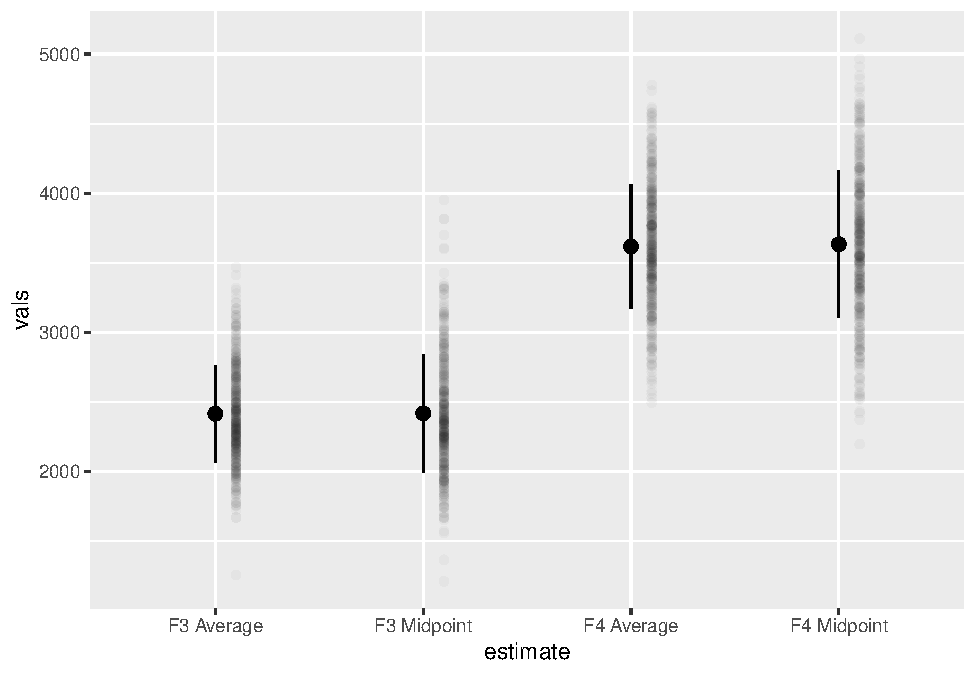
\includegraphics{paper_files/figure-latex/unnamed-chunk-4-1.pdf}
Across participants, pr06 (midpoint: 2090.85 Hz), pr08 (midpoint: 2194.17 Hz), pr09 (midpoint: 2207.76 Hz), and pr14 (midpoint: 2171.98 Hz) had the lowest F3 midpoint values. The F3 average for these participants was similarly lower. In contrast, pr04 (midpoint: 2872.95 Hz), pr05 (midpoint: 2565.45 Hz), and pr12 (midpoint: 2691.58 Hz) exhibited higher F3 values, generally above 2500 Hz. These participants also showed a higher average of F3, further confirming the higher frequency profile. Other participants, such as pr01 (midpoint: 2294.12 Hz), pr02 (midpoint: 2425.09 Hz), pr03 (midpoint: 2206.56 Hz), pr07 (midpoint: 2323.67 Hz), and pr13 (midpoint: 2456.46 Hz), showed F3 midpoint values in between the 2200-2450 Hz range, showing a middle ground between low and high F3 values.
F4 values, on the other hand, showed similar trends. Participants such as pr09 (midpoint: 3143.66 Hz), pr08 (midpoint: 3288.70 Hz), and pr14 (midpoint: 3621.00 Hz) showed lower F4 values, typically ranging from 3140 Hz to 3620 Hz for both midpoint and average values. In contrast, pr10 (midpoint: 4057.81 Hz), pr12 (midpoint: 4077.41 Hz), and pr13 (midpoint: 3917.43 Hz) showed higher F4 values, generally exceeding 3900 Hz for both their midpoint and average values. These participants showed a higher concentration of energy. In the end, for most participants, the difference between the F4 midpoint and F4 average was minimal, suggesting stable F4 production. However, participants like pr06 (midpoint: 3426.61 Hz, average: 3345.63 Hz) and pr08 (midpoint: 3288.70 Hz, average: 3219.33 Hz) exhibited a slightly larger difference, indicating some internal variation during /r/ production. (See Figure 2. for a more detailed description on F3 and F4 measurements across participants).

Figure 2.
Distribution of F3 and F4 across participants: Mean and Midpoint Frequencies

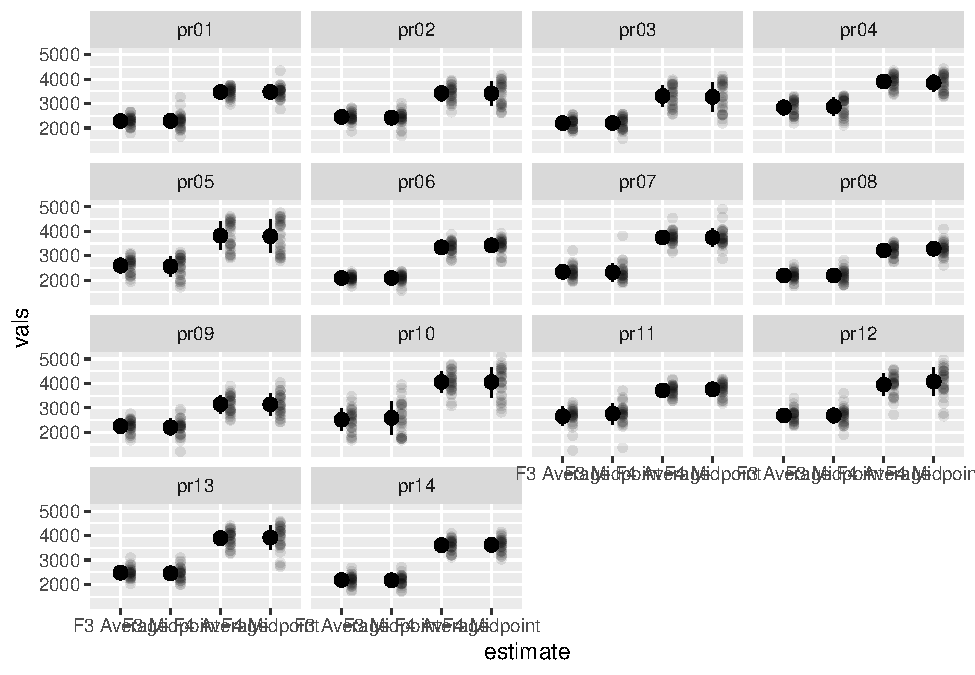
\includegraphics{paper_files/figure-latex/unnamed-chunk-5-1.pdf}
Overall, considering Luna's (2010) findings, which showed that lateralized /r/ sounds tend to have lower F3 and F4 values compared to canonical {[}l{]}, with average values for lateralized /r/ at approximately 2547 Hz (F3) and 3545 Hz (F4), it was possible to determine which participants in the current dataset showed more or less lateralization. Thus, participants such as pr06 (F3: 2090 Hz, F4: 3346 Hz), pr08 (F3: 2194 Hz, F4: 3219 Hz), pr09 (F3: 2254 Hz, F4: 3152 Hz), pr14 (F3: 2181 Hz, F4: 3606 Hz), pr03 (F3: 2203 Hz, F4: 3315 Hz), and pr01 (F3: 2289 Hz, F4: 3474 Hz) presented the lowest average F3 and F4 values, suggesting greater degrees of lateralization. On the other hand, participants pr04 (F3: 2846 Hz, F4: 3904 Hz), pr05 (F3: 2599 Hz, F4: 3822 Hz), pr10 (F3: 2516 Hz, F4: 4059 Hz), pr12 (F3: 2692 Hz, F4: 3951 Hz), and pr11 (F3: 2659 Hz, F4: 3716 Hz) showed less lateralization, with both F3 and F4 means clearly above the expected values for lateralized /r/. Participants like pr02 (F3: 2456 Hz, F4: 3430 Hz), pr07 (F3: 2341 Hz, F4: 3751 Hz), and pr13 (F3: 2480 Hz, F4: 3895 Hz) exhibited intermediate values, indicating a moderate or mixed degree of lateralization. This variation supports the idea of gradient lateralization across individuals.

\subsection{About the effect of internal and external linguistic factors on F3 and F4 values}\label{about-the-effect-of-internal-and-external-linguistic-factors-on-f3-and-f4-values}

To assess the influence of internal linguistic and external social factors on F3 values, a series of mixed-effects models were built with random intercepts for participants and lexical items. This approach accounts for repeated measures and individual variability while capturing the hierarchical structure of the data. It also allows for the simultaneous analysis of linguistic factors (e.g., word category, vowel context, word position) and social variables (e.g., gender, educational background) within a unified framework. Importantly, because position inside the word varies within individuals, I also included random slopes for this factor by participant. This approach captures possible differences in how each speaker is influenced by word position, and it aligns with best practices for modeling within-subject variation in mixed-effects frameworks.

\subsection{F3 Measurements}\label{f3-measurements}

To examine the factors influencing F3 production, I first ran a null model that included random intercepts for both participant and word, as well as a by-participant random slope for position inside the word. The fixed effect estimate indicated that the overall mean F3 value is approximately 2374.70 Hz, with a standard error of 61.13 and a significant p-value (p \textless{} 0.001).
Next, position inside the word (internal vs.~final) was added as a fixed effect (Model 1). The addition of this predictor significantly improved model fit compared to the null model (p = 0.015). In Model 1, F3 values were significantly higher when the segment occurred in word-internal position compared to word-final position (Estimate = 127.85, SE = 50.22, t(26.06) = 2.55, p = 0.018).
As a next step, word category (adjective, noun, preposition, verb) was introduced as an additional predictor (Model 2). However, this variable did not yield any significant effects (p \textgreater{} 0.24 for all comparisons), suggesting that word category did not meaningfully contribute to the prediction of F3 values.
As a result, preceding vowel was introduced as an alternative predictor alongside position inside the word (Model 3). The addition of preceding vowel significantly improved model fit relative to Model 1 (p = 0.005). Within Model 3, the vowel /o/ was associated with lower F3 values compared to other vowels (Estimate = --106.03, SE = 45.39, t(20.19) = --2.34, p = 0.030); the effect of /e/ was marginal (Estimate = 94.29, SE = 52.41, t(24.42) = 1.80, p = 0.084).
To evaluate the combined influence of internal and external factors on F3 values, a fourth model (Model 4) was built by adding gender as a fixed effect, alongside position inside the word and preceding vowel. While gender (women) approached marginal significance (Estimate = 219.26, SE = 104.24, t(12.00) = 2.10, p = 0.057), the inclusion of this predictor did not significantly improve model fit over Model 3 (p = 0.093). Nonetheless, to test whether gender interacted with preceding vowel quality, a fifth model (Model 5) was fitted with an interaction term (preceding vowel × gender). This model significantly outperformed all previous models (p \textless{} 0.001). The interaction between vowel /e/ and gender was highly significant (Estimate = 243.38, SE = 58.99, t(379.87) = 4.13, p \textless{} 0.001), demonstrating that the effect of /e/ on F3 values varied by gender. Additionally, a significant interaction was also found for vowel /o/ (Estimate = 126.85, SE = 61.77, t(379.87) = 2.05, p = 0.041), suggesting that gender also modulated the effect of /o/ on F3 values (see Figure 3 for a visual representation on the interaction between gender and preceding vowels).

Figure 3.
Interaction Between Gender and Preceding Vowel on F3 and F4 Values

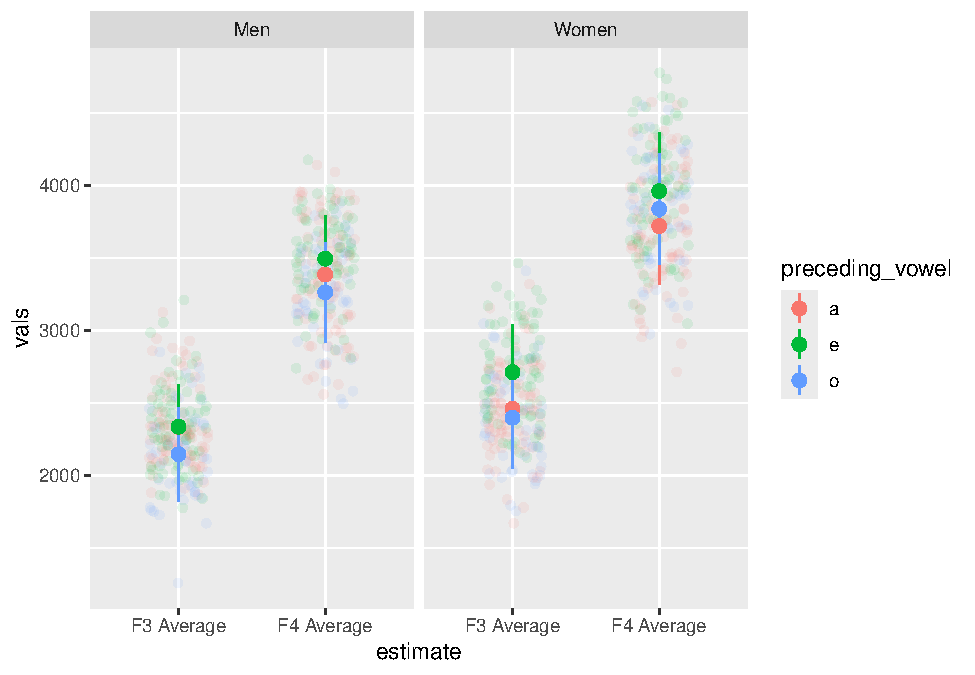
\includegraphics{paper_files/figure-latex/unnamed-chunk-6-1.pdf}
In the end, the anova function in R was also used to confirm that each step improved model fit: Model 1 (position inside the word) improved over the null model (p = 0.015), Model 3 (adding preceding vowel) improved over Model 1 (p = 0.005), Model 4 (adding gender) did not significantly improve over Model 3 (p = 0.093), and Model 5 (adding the interaction between vowel and gender) provided the best overall fit (p \textless{} 0.001).

While educational background was also considered as a potential external factor, uneven group sizes across education levels limited its inclusion in the models. As such, I consider it is more appropriate to describe general means and F3 midpoints across educational groups. Thus, the analysis of F3 values across educational backgrounds revealed a possible relationship between education level and F3 production. Participants with a master's degree showed the lowest and most consistent F3 values, with a mean F3 midpoint of 2148.71 Hz (SD = 229.01) and a mean F3 average of 2146.70 Hz (SD = 181.88). Those with a bachelor's degree showed higher and more variable F3 values (midpoint = 2413.65 Hz, SD = 397.03; average = 2410.02 Hz, SD = 337.65). Participants with a doctoral degree had slightly higher means (midpoint = 2496.26 Hz, SD = 412.27; average = 2506.37 Hz, SD = 333.25), indicating a trend toward elevated F3 frequencies. The highest values were observed in the high school category (midpoint = 2590.42 Hz, average = 2515.66 Hz), although this category included only one participant.

\subsection{F4 Measurements}\label{f4-measurements}

To examine the factors influencing the production of F4, I first ran a null model that included random intercepts for both participant and word, as well as a by-participant random slope for position inside the word. The fixed effect estimate indicated that the overall mean F4 value is approximately 3616.76 Hz, with a standard error of 80.13 and a highly significant p-value (p \textless{} 0.001).
Next, position inside the word (internal vs.~final) was added as a fixed effect (Model 1). This addition improved the model fit compared to the null model (p = 0.0099). In Model 1, F4 values were significantly higher when the segment occurred in word-internal position compared to word-final position, with an estimate of 150.41 Hz (SE = 54.45, t(15.89) = 2.76, p = 0.0139).\\
In Model 2, word category was added (adjective, noun, preposition, verb) as an additional predictor. The results revealed that prepositions were associated with a significantly lower F4 compared to adjectives (Estimate = --315.18, SE = 109.32, t(19.73) = --2.88, p = 0.0093). Nonetheless, these results should be understood carefully because there was only one token for prepositions. Other word categories (noun, verb) did not significantly affect F4. Specifically, the coefficient for nouns (Estimate = --31.71, SE = 51.02, t(12.76) = --0.62, p = 0.5451) and verbs (Estimate = --48.09, SE = 55.19, t(13.51) = --0.87, p = 0.3987) were not significant.

In Model 3, both position inside the word and preceding vowel were included. The intercept was 3543.16 (SE = 84.90, p \textless{} 0.001). The effect of position inside the word (internal) was not significant (Estimate = 61.66, SE = 65.16, p = 0.354), while preceding vowel /e/ significantly increased F4 values (Estimate = 126.45, SE = 58.30, p = 0.041). Preceding /o/ had no effect (Estimate = --7.59, SE = 49.43, p = 0.880).
To evaluate the combined influence of internal and external factors on F4 values, a fourth model (Model 4) was built by adding gender as a fixed effect, alongside position inside the word and preceding vowel. In this model, the intercept dropped slightly to 3314.50 (SE = 81.97, p \textless{} 0.001). The effect of gender was highly significant (Estimate = 457.31, SE = 100.51, p \textless{} 0.001), demonstrating that women had higher F4 values. The effect of /e/ remained significant (Estimate = 126.45, SE = 58.30, p = 0.041), while position inside the word (Estimate = 61.66, SE = 65.16, p = 0.354) and /o/ (Estimate = --7.59, SE = 49.43, p = 0.880) remained non-significant.

Model 5 tested interaction between preceding vowel and gender. The intercept was 3363.96 (SE = 86.34, p \textless{} 0.001). The main effect of gender (women) remained significant (Estimate = 358.38, SE = 113.76, p = 0.0057), and the interaction between /o/ and gender was also significant (Estimate = 241.83, SE = 81.83, p = 0.0033). This suggests that preceding /o/ lowered F4 for men, but not for women. The interaction between /e/ and gender was not significant (Estimate = 108.16, SE = 83.67, p = 0.198) (see Figure 3. For a better description).
In the end, the anova function in R was also used to confirm that each step improved model fit. Model 1 showed significant improvement (p = 0.0099). Model 3 was marginally better than Model 1 (p = 0.067), and Model 4 significantly improved model fit (p \textless{} 0.0001). Model 5 also provided a significant improvement over Model 4 (p = 0.0127), largely driven by the interaction with the preceding vowel /o/, which had a significant effect when combined with gender.
As with F3, educational background was also considered as a potential external factor in the analysis of F4. Overall, descriptive results reveal notable variation across groups: the high school participant showed the highest F4 values (midpoint mean = 4057.81 Hz; average = 4058.86 Hz), while speakers with a master's degree exhibited the lowest F4 values (midpoint mean = 3351.07 Hz; average = 3330.08 Hz). This might suggest a potential downward trend in F4 with higher education levels, although the doctoral group had slightly higher values than both the bachelor's and master's groups (midpoint mean = 3659.08 Hz; average = 3676.04 Hz).

Overall, both the F3 and F4 measurements revealed that internal linguistic factors (such as position inside the word and preceding vowel) and external social factors (particularly gender) significantly influenced acoustic outcomes, though the strength and nature of these effects varied across the two formants. For both F3 and F4, the segment's position inside the word had a consistent effect, with word-internal position with higher values. Preceding vowel also played a role in both cases: vowel /o/ lowered F3 but had no significant effect on F4, while vowel /e/ showed a marginal or significant raising effect on both, particularly when interacting with gender. Gender emerged as a strong predictor in both models, with women producing higher F3 and F4 values, and its interaction with vowel quality (especially /e/ and /o/) significantly improved model fit for both formants. Educational background was descriptively linked to both F3 and F4 trends (lower frequencies in more educated participants), but group imbalances prevented formal statistical testing.

\section{Discussion}\label{discussion}


\end{document}
